% Figure 1 — The workflow of the sequential hybrid sampling framework.
% Build (dari manuscript/latex/):
%   pdflatex -output-directory=figures figures/F0_framework.tex
%   cp figures/F0_framework.pdf ../F0_framework.pdf
\documentclass[tikz,border=8pt]{standalone}
\usetikzlibrary{arrows.meta,positioning,decorations.pathreplacing,calc}

\begin{document}
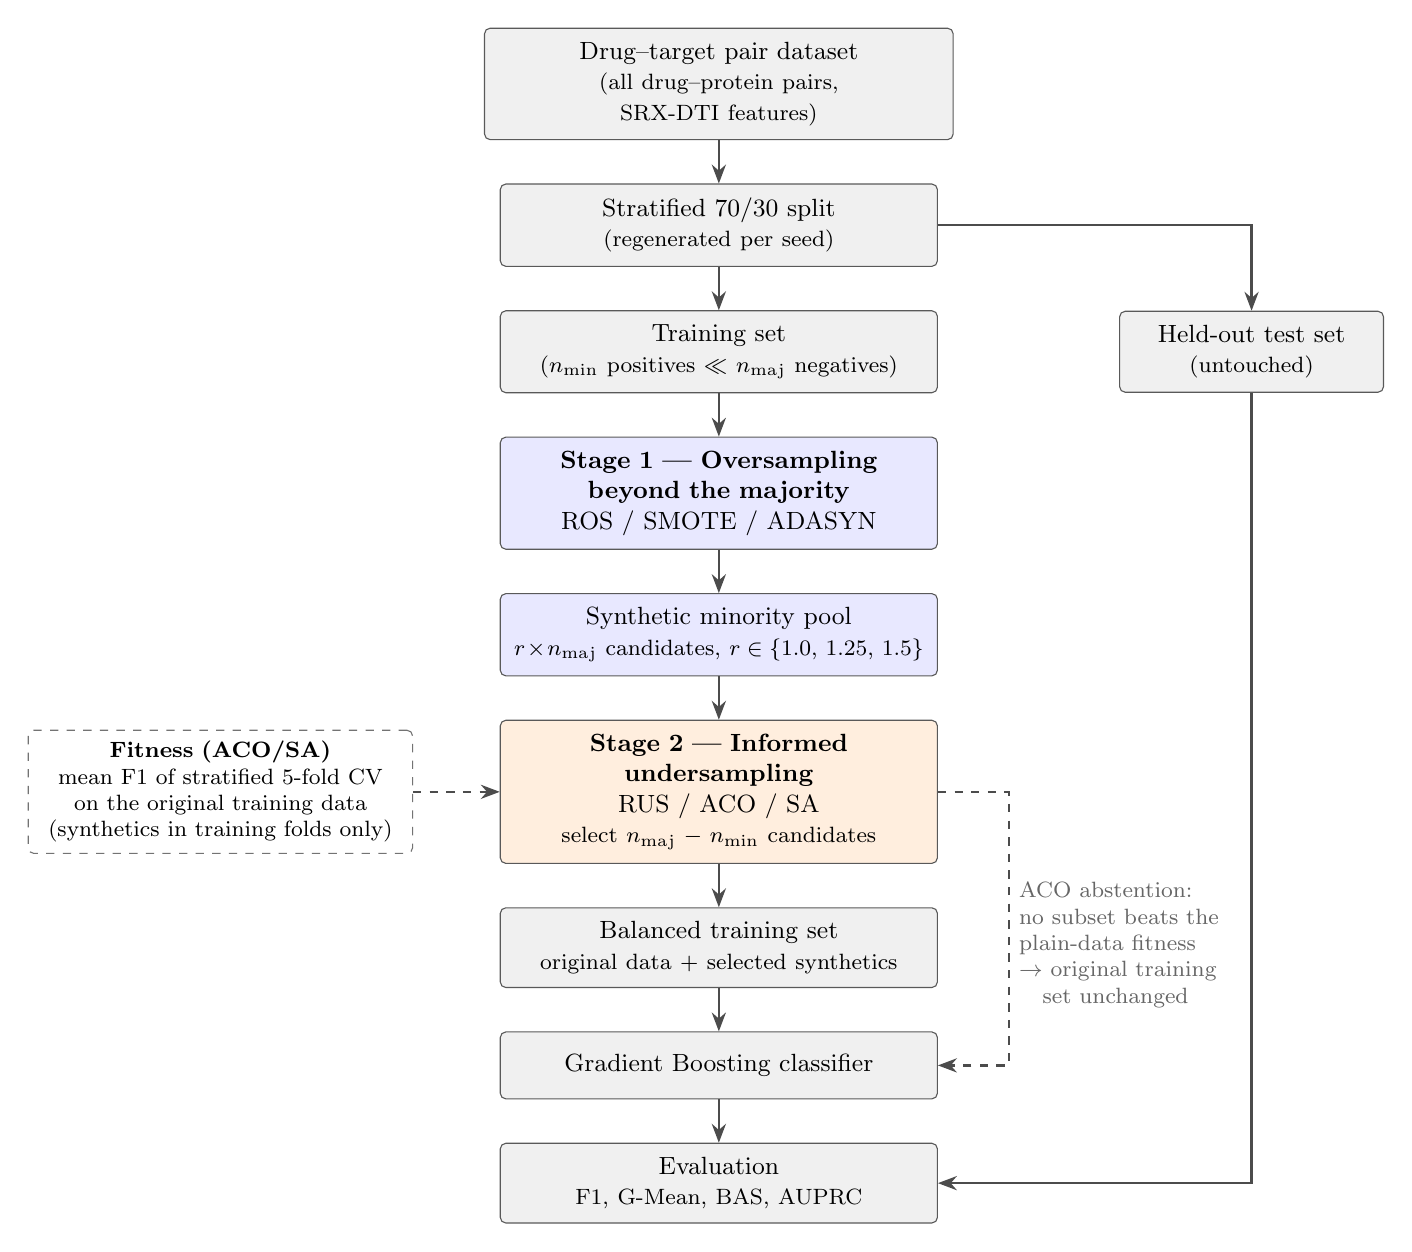
\begin{tikzpicture}[
  font=\small,
  node distance=5.5mm and 9mm,
  box/.style={draw=black!65, rounded corners=2pt, align=center,
              inner sep=5pt, text width=52mm, minimum height=8.5mm},
  data/.style={box, fill=black!6},
  proc1/.style={box, fill=blue!9},
  proc2/.style={box, fill=orange!13},
  side/.style={draw=black!55, dashed, rounded corners=2pt, align=center,
               inner sep=4pt, text width=46mm, fill=white, font=\footnotesize},
  arr/.style={-{Stealth[length=2.4mm]}, thick, black!70},
  dasharr/.style={arr, dashed},
  lbl/.style={font=\footnotesize\itshape, black!60},
]

% ---------- main flow ----------
\node[data, text width=56mm] (dataset) {Drug--target pair dataset\\
  \footnotesize (all drug--protein pairs, SRX-DTI features)};
\node[data, below=of dataset] (split) {Stratified 70/30 split\\
  \footnotesize (regenerated per seed)};
\node[data, below=of split] (train) {Training set\\
  \footnotesize ($n_{\min}$ positives $\ll$ $n_{\mathrm{maj}}$ negatives)};

\node[proc1, below=of train] (ovs)
  {\textbf{Stage 1 --- Oversampling beyond the majority}\\
  ROS / SMOTE / ADASYN};
\node[proc1, below=of ovs] (pool) {Synthetic minority pool\\
  \footnotesize $r \times n_{\mathrm{maj}}$ candidates,
  $r \in \{1.0,\,1.25,\,1.5\}$};

\node[proc2, below=of pool] (sel)
  {\textbf{Stage 2 --- Informed undersampling}\\
  RUS / ACO / SA\\
  \footnotesize select $n_{\mathrm{maj}} - n_{\min}$ candidates};

\node[data, below=of sel] (bal) {Balanced training set\\
  \footnotesize original data $+$ selected synthetics};
\node[data, below=of bal] (clf) {Gradient Boosting classifier};
\node[data, below=of clf] (eval) {Evaluation\\
  \footnotesize F1, G-Mean, BAS, AUPRC};

\draw[arr] (dataset) -- (split);
\draw[arr] (split) -- (train);
\draw[arr] (train) -- (ovs);
\draw[arr] (ovs) -- (pool);
\draw[arr] (pool) -- (sel);
\draw[arr] (sel) -- (bal);
\draw[arr] (bal) -- (clf);
\draw[arr] (clf) -- (eval);

% ---------- fitness side box (left of selector) ----------
\node[side, left=of sel, xshift=-2mm] (fit) {\textbf{Fitness (ACO/SA)}\\
  mean F1 of stratified 5-fold CV\\ on the original training data\\
  (synthetics in training folds only)};
\draw[dasharr] (fit) -- (sel);

% ---------- test-set path (right side) ----------
\node[data, right=of train, xshift=14mm, text width=30mm] (test)
  {Held-out test set\\ \footnotesize (untouched)};
\draw[arr] (split.east) -| (test.north);
\draw[arr] (test.south) |- (eval.east);

% ---------- ACO abstention bypass ----------
\coordinate (bypass) at ($(sel.east)+(9mm,0)$);
\draw[dasharr] (sel.east) -- (bypass) |- (clf.east)
  node[pos=0.28, right, align=left, font=\footnotesize, black!60]
  {ACO abstention:\\ no subset beats the\\ plain-data fitness\\
   $\rightarrow$ original training\\ \quad set unchanged};

\end{tikzpicture}
\end{document}
